\documentclass[a4paper,12pt]{article}


\usepackage[MeX]{polski}
\usepackage[utf8]{inputenc}	% kodowanie znaków
\usepackage{indentfirst}

\usepackage{upquote}  	% zamiana cudzysłowów klasycznych (,, ") na górne (" ") w kodach źródłowych
\usepackage{graphicx}	% wstawianie obrazków
\usepackage{amsmath}
\usepackage{listings}
\usepackage{color}
\usepackage{xcolor}


\def\PICSDIR{PICS}

% Ustawienie marginesów
\oddsidemargin=0.5cm
\evensidemargin=-0.5cm
\topmargin=0cm
\textwidth=16cm
\textheight=23cm


\frenchspacing

\clubpenalty=10000		% to kara za sierotki
\widowpenalty=10000		% nie pozostawia wdów
\brokenpenalty=10000 	% nie dzieli wyrazów pomiędzy stronami


\sloppy

\usepackage{caption}
\captionsetup{
	margin=10pt,
	font=small,
	labelfont=bf
}

% Pakiety z ładnymi czcionkami
\usepackage[T1]{fontenc}
\usepackage{lmodern}


% Ładniejsze tabelki
\usepackage{booktabs}

% Ustawienia wyglądu listingów
\lstset{
	language=C++,                               % choose the default language of the code
	basicstyle=\footnotesize\ttfamily,       	% the size of the fonts that are used for the code
	numbers=left,                   		% where to put the line-numbers
	numberstyle=\tiny,      			% the size of the fonts that are used for the line-numbers
	stepnumber=1,                   		% the step between two line-numbers. If it's 1 each line will be numbered
	numbersep=5pt,                  		% how far the line-numbers are from the code
	showspaces=false,               		% show spaces adding particular underscores
	showstringspaces=false,         	% underline spaces within strings
	showtabs=false,                 		% show tabs within strings adding particular underscores
	tabsize=4,	                		% sets default tabsize
	captionpos=b,                   		% sets the caption-position
	breaklines=true,                		% sets automatic line breaking
	breakatwhitespace=true,        	% sets if automatic breaks should only happen at whitespace
	extendedchars=true,
	keywordstyle=\bfseries\color[RGB]{0,0,127},
	identifierstyle=,
	commentstyle=\color[RGB]{90,90,90}\slshape,
	stringstyle=\slshape,
	xleftmargin=30pt,
	frame=tb,
	framexleftmargin=30pt,
	emph=
	{[1]
		uint8_t, uint32_t, aes_state_t
	},
	emphstyle={[1]\color[RGB]{0,127,0}},
	emph=
	{[2]
		aesCipherCounter, aesInitGlobalData, aesKeyExpansion, aesCipherT
	},
	emphstyle={[2]\color[RGB]{0,127,127}},
	emph=
	{[3]
		MPI_Bcast, MPI_Scatter, MPI_Gather
	},
	emphstyle={[3]\color[RGB]{127,0,127}},
	emph=
	{[4]
		MPI_BYTE, MPI_INT, MPI_COMM_WORLD
	},
	emphstyle={[4]\color[RGB]{127,0,0}\slshape},
}

\begin{document}

\title{{\small Programowanie równoległe i rozproszone}\\Algorytm szyfrujący AES w trybie CTR}
\author{Maciej Stefańczyk, Kacper Szkudlarek}

\maketitle

\begin{abstract}
Dokumentacja realizacji projektu z przedmiotu ,,Programowanie równoległe i~rozproszone''. W ramach projektu wykonana została implementacja algorytmu szyfrującego AES (Advanced Encryption Standard) pracującego w trybie CTR (Counter mode). Zrównoleglenie zostało oparte o bibliotekę OpenMP dla pamięci wspólnej, oraz MPI dla pamięci rozproszonej.
\end{abstract}


\section{Wstęp}
Algorytm szyfrujący AES (ang. Advanced Encryption Standard) jest to symetryczny szyfr blokowy przyjęty przez NIST (ang. National Institute of Standards and Technology) jako standard szyfrowania. Algorytm został stworzony w ramach ogłoszonego konkursu, który miał wyłonić następcę algorytmu DES(ang. Data Encryption Standard). Jego robocza nazwa to Rijndael. Ze względu na swą złożoność algorytm uważany jest za bezpieczny i powszechnie stosowany.

Algorytm szyfruje i deszyfruje dane w 128-bitowych blokach, korzystając z 128, 192 lub 256 bitowych kluczy. Dane, na których operuje algorytm formowane są w macierz 4x4, w której każda komórka jest jednym bajtem danych. W zależności do wybranej wielkości klucza szyfrującego wykonywane jest odpowiednio 10, 12 lub 14 rund szyfrujących. Wszystkie rundy poza pierwszą i ostatnią składają się z czterech kroków:
\begin{enumerate}
\item Etap: zamiana wstępna -- jest to nielinowe przekształcenie każdego bajtu poprzez zamianę jego wartości zgodnie z tablicą LUT.
\item Etap: zamiana wierszy -- na każdym wierszu danych wykonywana jest operacja rotacji cyklicznej o zadaną liczbę pozycji.
\item Etap: mieszanie kolumn -- każda kolumna poddawana jest odwracalnej liniowej transformacji.
\item Etap: dodanie klucza rundowego -- do danych dodawany jest klucz rundowy wygenerowany na podstawie klucza głównego.
\end{enumerate}

W opisywanej implementacji algorytm szyfrowania AES pracował w trybie CTR (od ang. counter, tryb licznikowy). Pozwala wykorzystać on szyfry blokowe do kodowania m.in. strumieni danych. Generowany jest pseudolosowy ciąg danych, który pełni rolę strumienia szyfrującego. Jest on mieszany poprzez użycie operacji XOR z danymi wejściowymi, przez co uzyskujemy zaszyfrowany ciąg danych. Zostało to przedstawione na rysunku~\ref{rys:ctr}. Ważną cechą trybu CTR jest wykorzystywanie jedynie operacji szyfrowania (także przy odszyfrowywaniu danych), odszyfrowywanie wykorzystuje własność operacji XOR.

\begin{figure}
\centering
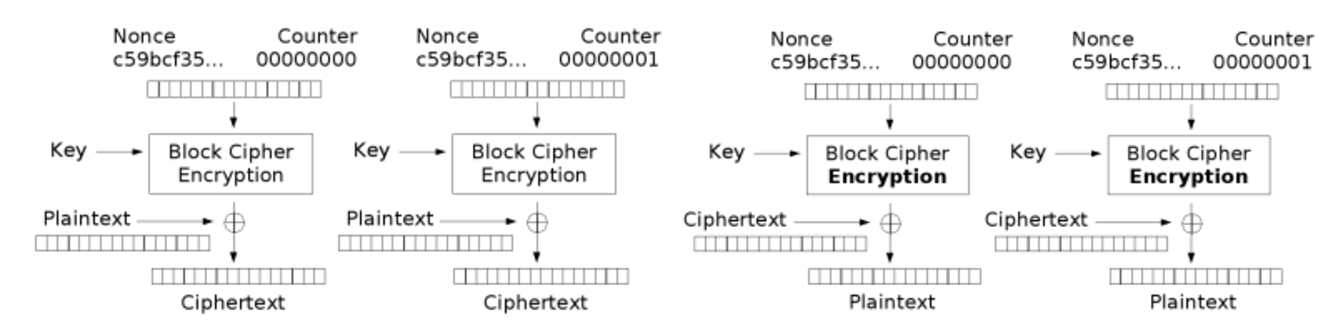
\includegraphics[width=\textwidth]{\PICSDIR/CTR_mode.pdf}
\caption{Schemat działania trybu licznikowego (po lewej szyfrowanie, po prawej odszyfrowywanie)}
\label{rys:ctr}
\end{figure}

\section{Implementacja}
W ramach projektu powstały trzy wersje oprogramowania opisane w dalszych paragrafach:
\begin{enumerate}
\item Wersja sekwencyjna -- jest to implementacja algorytmu w języku C wykonująca się jednowątkowo w sposób sekwencyjny.
\item Wersja wykorzystująca pamięć współdzieloną -- jest to rozwinięcie wersji sekwencyjnej, które dzięki wykorzystaniu OpenMP pozwala na równoległe wykonywanie na wielu procesorach.
\item Wersja wykorzystująca pamięć rozproszoną -- jest to rozwinięcie wersji sekwencyjnej, które dzięki wykorzystaniu biblioteki MPI pozwala na równoległe wykonywanie na wielu maszynach pracujących w ramach klastra obliczeniowego.
\end{enumerate}



\subsection{Wersja sekwencyjna}

Diagram przepływu danych dla stworzonej aplikacji został przedstawiony na rysunku~\ref{rys:da}.  Na podstawie danych podanych w wierszu poleceń w czasie wykonywania programu podejmowane są decyzje o trybie działania -- szyfrowanie, deszyfrowanie, długość wykorzystanego klucza, oraz pobierane są dane wejściowe.

Dane podawane do programu (klucz, dane do szyfrowania/deszyfrowania) odczytywane są bezpośrednio z plików i wczytywane w całości do pamięci. Dzięki takiemu rozwiązaniu narzut czasowy związany z odczytem i zapisem danych w czasie ich szyfrowania jest stosunkowo niewielki, gdyż wszystkie operacje przeprowadzane są na pamięci, a nie na plikach dyskowych. Powoduje to jednak wydłużenie czasu wczytywania danych, zwłaszcza przy dużych zbiorach, które maja być zaszyfrowane.

Pseudolosowa liczba wykorzystywana w trybie CTR do szyfrowania strumienia danych została zaimplementowana w postaci złożenia czterech 32 bitowych bloków. Najbardziej znaczące 32 bit wypełniane jest wartością czasu odczytaną w momencie ładowania do pamięci pliku z danymi do zaszyfrowania. Kolejne dwa bloki 32 bitowe stanowią liczby odpowiednio 1 i 0. Do najmniej znaczących 32 bit wpisywana jest wartość licznika zliczającego ilość zaszyfrowanych bloków. W czasie zapisywania wyników wartość górnych 64~bitów zapisywana jest na samym początku pliku wynikowego.

Wykorzystane w środkowej części liczy pseudolosowej wartości 1 i 0 w celu zwiększenia bezpieczeństwa należałoby zastąpić jakimiś bardziej skomplikowanymi wartościami.

W celu optymalizacji przetwarzania danych zostały wprowadzone pewne modyfikacje w sposobie przechowywania i zapisywania macierzy stanu algorytmu. Każda kolumna przechowywana jest w pamięci w postaci 32 bitowej liczby. Takie potraktowanie kolumn pozwoliło znacząco ułatwić proces ,,mieszania'' kolumn w trakcie szyfrowania.

\begin{figure}
\centering
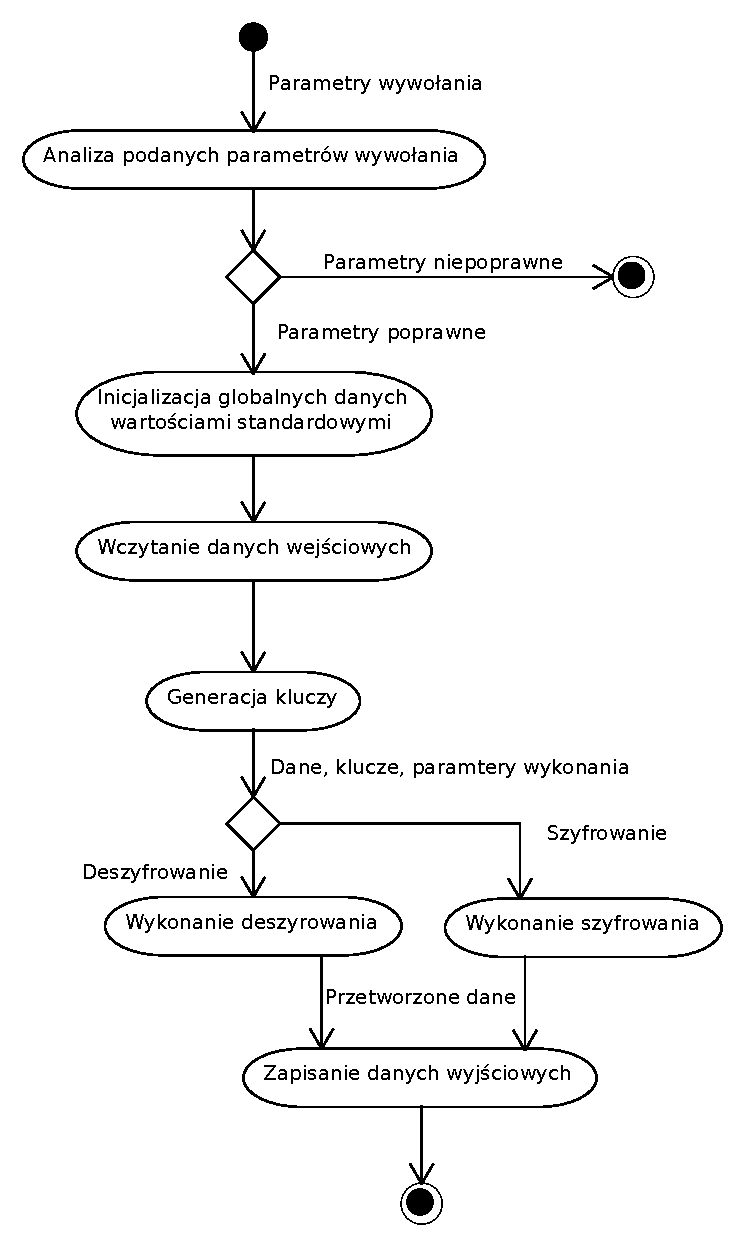
\includegraphics[width=\textwidth, height=0.95\textheight]{\PICSDIR/diagram_aktywnosci.pdf}
\caption{Diagram przepływu danych w czasie wywołanie programu.}
\label{rys:da}
\end{figure}

\subsection{Pamięć wspólna -- OpenMP}
\textbf{OpenMP} (ang. Open Multi-Processing)  jest to wieloplatformowy interfejs programowania aplikacji umożliwiający tworzenie aplikacji dla systemów wieloprocesorowych korzystających z pamięci współdzielonej. Interfejs może być wykorzystywany w językach C, C++ i FORTRAN, w systemach zarówno z rodziny Unix, Linux jak i Windows. Do sterowania sposobem wykonywania programu używa się zbioru dyrektyw preprocesora oraz zmiennych środowiskowych.

Dzięki zastosowaniu trybu licznikowego (CTR) w implementacji algorytmu AES możliwe było bardzo dobre zrównoleglenie przeprowadzanych obliczeń. W tym trybie każdy 128 bitowy blok danych szyfrowany jest niezależnie od pozostałych. Jedynym elementem, który należy kontrolować jest takie modyfikowanie licznika, by możliwe było późniejsze odtworzenie jego pracy w celu odszyfrowania danych.

W celu oznaczenia bloku do zrównoważenia użyta została dyrektywa preprocesora \texttt{omp parallel for}:
\begin{lstlisting}[language=c++]
#pragma omp parallel for default(none) private(i) shared(data, in_blocks, in_ptr32)
for (i = 0; i < in_blocks; ++i)
{
	aes_state_t ctr = aesCipherCounter(data, i);
	uint32_t c0 = *(uint32_t*)ctr.s;
	uint32_t c1 = *(uint32_t*)ctr.s+4;
	uint32_t c2 = *(uint32_t*)ctr.s+8;
	uint32_t c3 = *(uint32_t*)ctr.s+12;
	in_ptr32[4 * i    ] = in_ptr32[4 * i    ] ^ c0;
	in_ptr32[4 * i + 1] = in_ptr32[4 * i + 1] ^ c1;
	in_ptr32[4 * i + 2] = in_ptr32[4 * i + 2] ^ c2;
	in_ptr32[4 * i + 3] = in_ptr32[4 * i + 3] ^ c3;
}
\end{lstlisting}

Dyrektywa ta definiuje prywatne i współdzielone zmienne zawarte w wyróżnionym fragmencie. Jako prywatna została oznaczona zmienna sterująca pętla \texttt{for}, tak by każdy wątek mógł niezależnie przetwarzać dane. Zmiennymi publicznymi są natomiast:
\begin{itemize}
\item \texttt{data} -- struktura danych zawierająca zmienne globalne,
\item \texttt{in\_blocks} -- liczba bloków, które należy przetworzyć,
\item \texttt{in\_ptr32} -- wskaźnik na dane (dane zaszyfrowane są zapisywane w tym samym miejscu, z którego zsotały odczytane)
\end{itemize}

Zrównoleglona pętla \texttt{for} odpowiada za szyfrowanie algorytmem AES kolejnych 
chwilowych zmiennych losowych i przeprowadzanie operacji XOR tych zmiennych 
z szyfrowanymi danymi, a także operację odwrotną -- deszyfrowanie. Tak 
przetworzone dane są przekazywane do zapisania w pliku wynikowym.

\subsection{Pamięć rozproszona -- MPI}
\textbf{MPI} (ang. Message Passing Interface) jest to biblioteka będąca 
standardem przesyłania komunikatów w rzeczywistych i wirtualnych maszynach 
równoległych z pamięcią lokalną.

Przy użyciu MPI powstała wersja programu umożliwiająca zrównoleglenie obliczeń  
w oparciu o klaster.  Każdy z komputerów wchodzących w skład klastra dostaje 
porcję danych, którą przetwarza a następnie zawraca wyniki do procesu nadrzędnego.

Wykorzystywany jest komunikator \texttt{MPI\_COMM\_WORLD} obejmujący wszystkie procesy, które mogą między sobą wymieniać dane. Odczytywana jest ilość komputerów w komunikatorze i dla każdego procesu jego id w tym komunikatorze. Następnie następuje przetworzenie danych, co zostało przedstawione na listingu.

\begin{lstlisting}
// broadcast global data to all processes
MPI_Bcast(&key_size, 1, MPI_INT, root, MPI_COMM_WORLD);
MPI_Bcast(&direction, 1, MPI_INT, root, MPI_COMM_WORLD);
MPI_Bcast(genkey, key_size/8, MPI_BYTE, root, MPI_COMM_WORLD);
MPI_Bcast(&data.in_blocks, 4, MPI_BYTE, root, MPI_COMM_WORLD);
MPI_Bcast(&data.nonce_0, 4, MPI_BYTE, root, MPI_COMM_WORLD);
MPI_Bcast(&data.nonce_1, 4, MPI_BYTE, root, MPI_COMM_WORLD);

aesInitGlobalData(&data, key_size);

// allocate data buffer for each process
data.in_data = malloc(data.in_blocks * data.block_size);
aesKeyExpansion(&data, genkey);


// scatter data to all processes
MPI_Scatter(input_buffer, data.in_blocks*data.block_size, MPI_BYTE, data.in_data,  data.in_blocks*data.block_size, MPI_BYTE, root, MPI_COMM_WORLD);

// process data - cipher/decipher given block
aesCipherT(&data);

// return processed data
MPI_Gather(data.in_data, data.in_blocks*data.block_size, MPI_BYTE, input_buffer,  data.in_blocks*data.block_size, MPI_BYTE, root, MPI_COMM_WORLD);
\end{lstlisting}

Do każdego procesu wysyłane są zmienne globalne, takie jak wielkość używanego klucza, 
klucz, kierunek pracy (szyfrowanie/deszyfrowanie danych), ilość wszystkich bloków 
do przetworzenia, a także wygenerowana wartość używana w czasie tworzenia zmiennej tymczasowej.
Następnie każdy z procesów alokuje sobie pamięć dla danych, które będzie przetwarzał. 
Przy użyciu funkcji \texttt{MPI\_Scatter} dane wejściowe aplikacji zostają podzielone 
i rozesłane do poszczególnych procesów, gdzie następuje ich przetworzenie (jak 
w~wersji sekwencyjnej, wykorzystywany jest ten sam kod). Po zakończeniu przetwarzania 
wszystkie procesy odsyłają dane przy pomocy funkcji \texttt{MPI\_Gather}, 
a proces nadrzędny zapisuje je do pliku wynikowego.

\subsection{Obsługa programu}

Niezależnie od wersji (OpenMP bądź MPI) program posiada taki sam zestaw parametrów, 
które należy do niego podać. Program wywoływany jest poleceniem:\\
\texttt{aes\_ctr [OPCJE] nazwa\_pliku\_wejsciowego}, gdzie opcje mogą przyjmować
następujące wartości:

\begin{description}
\item[\texttt{-s [128|192|256]}] \hfill \\ 
Długość klucza
\item[\texttt{-g path}] \hfill \\ 
Ścieżka do pliku zawierającego plugin generujący klucz właściwy
\item[\texttt{-k string}] \hfill \\ 
Klucz
\item[\texttt{-o path}] \hfill \\ 
Nazwa pliku wynikowego
\item[\texttt{-[c|d]}] \hfill \\ 
Szyfrowanie/deszyfrowanie
\item[\texttt{-v}] \hfill \\ 
Tryb gadatliwy -- wypisywanie pośrednich informacji
\end{description}

Dodatkowych wyjaśnień może wymagać generowanie klucza -- w celu zamiany podanego
klucza (w postaci napisu) na odpowiedniej długości klucz właściwy, wykorzystywane
są dodatkowe pluginy. W chwili obecnej zaimplementowana jest jedynie biblioteka
wykorzystująca algorytm MD5.

\section{Testy}

\subsection{Testy jednostkowe}

Testy jednostkowe mają za zadanie wykazanie poprawności działania poszczególnych elementów składowych tworzonego oprogramowania.  Dla opisywanej aplikacji powstały następujące testy:
\begin{enumerate}
\item \textbf{\texttt{test\_key}} -- jest to test badający poprawność generowanych kluczu rundowych. Do funkcji podawane są dane testowe w postaci klucza pierwotnego, rozmiaru klucza, a także oczekiwanego wyniku. Funkcja testuje poprawność wygenerowanego klucza porównując go z podanym oczekiwanym wynikiem.
\item \textbf{\texttt{test\_mix}} -- jest to funkcja testująca mieszanie kolumn macierzy stanu algorytmu szyfrującego. Pobiera dwa argumenty, pierwszym jest przykładowa macierz stanu, drugim oczekiwane rezultaty. Po wykonaniu operacji mieszania otrzymane wyniki porównywane są z otrzymanymi danymi.
\item \textbf{\texttt{test\_shift}} -- jest to funkcja testująca poprawność operacji rotacji wierszy macierzy stanu algorytmu. Podobnie jak funkcja \texttt{test\_mix} pobiera dwa argumenty -- przykładową macierz stanu i oczekiwany wynik operacji, z którym porównywane są otrzymane wyniki.
\item \textbf{\texttt{test\_ctr}} -- jest to test badający poprawność szyfrowania zaimplementowanego algorytmu. Jako dane wejściowe pobierane są wektor inicjujący, dane do zaszyfrowania, oczekiwane wyniki oraz klucz, który ma być użyty do szyfrowania. Wektor użyty w~tym teście jednostkowym został pobrany z publikacji NIST ,,Recommendation for Block Cipher Modes of Operation''.
\end{enumerate}

\subsection{Testy wydajności}

Drugim wykonanym rodzajem testów stworzonej aplikacji są testy wydajnościowe. Zadaniem testów było zmierzenie różnic w czasie wykonania tego samego zadania testowego przez różne wersje oprogramowania. Wyniki testów jednoznacznie pokazały wzrost wydajności aplikacji poprzez użycie narzędzi do zrównoleglania obliczeń.

\subsubsection{Dane testowe}

Do testowania stworzonych aplikacji wykorzystany został skrypt przedstawiony na wydruku~\ref{lst_testthread}.
\begin{lstlisting}[label=lst_testthread,caption={Skrypt testowy (wersja OpenMP, 
wersja MPI różni się jedynie wywołaniem mpiexec zamiast prostego wywołania programu)},language=bash]
#!/bin/bash

# set size of test file
if [ -n "$1" ]
then
	filesize=$1
else
	filesize=10
fi

# set number of cipher/decipher repeats for each thread count
if [ -n "$2" ]
then
	repeats=$2
else
	repeats=10
fi

# set maximum number of threads allowed
if [ -n "$3" ]
then
	max_threads=$3
else
	max_threads=16
fi

# generate random test file of given size
filename=randomfile

echo "Generating random $filesize MB test file"
dd if=/dev/urandom of=$filename bs=1M count=$filesize

# test program for each allowed number of threads (1, 2, 4, 8, ...)
echo "Testing OpenMP ($repeats repeats, max $max_threads threads)..."
for (( t=1; t<=$max_threads; t*=2 ))
do
	echo "$t threads..."
	export OMP_NUM_THREADS=$t
	
	for (( c=1; c<=$repeats; c++ ))
	do
		./aes_ctr -c -g ../lib/libhash_md5.so -k 1234 -o $filename.out -s 128 $filename
		./aes_ctr -d -g ../lib/libhash_md5.so -k 1234 -o $filename.or -s 128 $filename.out
		diff randomfile randomfile.or
	done

done

# remove temporary files
rm $filename 
rm $filename.or
rm $filename.out
\end{lstlisting}

Skrypt wywoływany jest poleceniem:\\
\texttt{./test\_threads.sh [TEST\_SIZE [REPEATS [THREADS]]]}

Plik testowy generowany jest przy użyciu systemowego generatora liczb pseudolosowych, 
jako że zawartość pliku nie ma żadnego wpływu na szybkość szyfrowania. Wygenerowany
plik jest następnie określoną liczbę razy szyfrowany i deszyfrowany, a wyniki są 
porównywane (plik przez zaszyfrowaniem z plikiem po odszyfrowaniu). Cykl ten jest 
powtarzany dla zwiększającej się liczby wątków, aż do maksymalnej, określonej liczby.

\subsubsection{Wyniki -- OpenMP}

Pierwsze przedstawione zostaną wyniki dla wersji OpenMP. Testy przeprowadzone 
zostały na maszynie z ośmioma dwurdzeniowymi procesorami AMD Opteron 8218 2,6GHz.

W tabeli~\ref{tab:omp}
zebrane zostały wyniki pomiarów dla pliku testowego wielkości 10MB. Oznaczenia:
\begin{itemize}
\item $p$ -- liczba wątków,
\item $T_s(p)$ -- czas wykonania części sekwencyjnej przy podziale na $p$ wątków,
\item $T_p(p)$ -- czas wykonania części równoległej przy podziale na $p$ wątków,
\item $T(p)$ -- całkowity czas wykonania programu przy podziale na $p$ wątków,
\item $E(p)$ -- wydajność samej operacji szyfrowania,
\item $S_p(p)$ -- przyspieszenie części równoległej,
\item $S(p)$ -- przyspieszenie całego programu.
\end{itemize}


\begin{table}[h!]
\caption{Czas przetwarzania danych w wersji OpenMP}
\centering
\footnotesize
\begin{tabular}{rrrrrrr}
\toprule
$p$&$T_s(p)$&$T_p(p)$&$T(p)$&$E(p)$&$S_p(p)$&$S(p)$\\
\cmidrule{1-7}
&ms&ms&ms&MB/s&&\\
\midrule
 1 & 79,27 & 493,34 & 572,61 &  20,27 &  1,00 & 1,00\\
 2 & 67,82 & 247,44 & 315,26 &  40,41 &  1,99 & 1,82\\
 4 & 69,80 & 123,79 & 193,59 &  80,79 &  3,99 & 2,96\\
 6 & 69,79 &  82,85 & 152,63 & 120,70 &  5,95 & 3,75\\
 8 & 70,39 &  62,28 & 132,67 & 160,58 &  7,92 & 4,32\\
10 & 68,92 &  50,05 & 118,97 & 199,78 &  9,86 & 4,81\\
12 & 69,29 &  41,79 & 111,08 & 239,27 & 11,80 & 5,15\\
14 & 69,54 &  36,05 & 105,60 & 277,36 & 13,68 & 5,42\\
16 & 69,45 &  31,85 & 101,29 & 314,00 & 15,49 & 5,65\\
\bottomrule
\end{tabular}
\label{tab:omp}
\end{table}

Wykres~\ref{rys:res_omp} przedstawia w sposób obrazowy uzyskane wyniki.

\begin{figure}[h!]
\centering
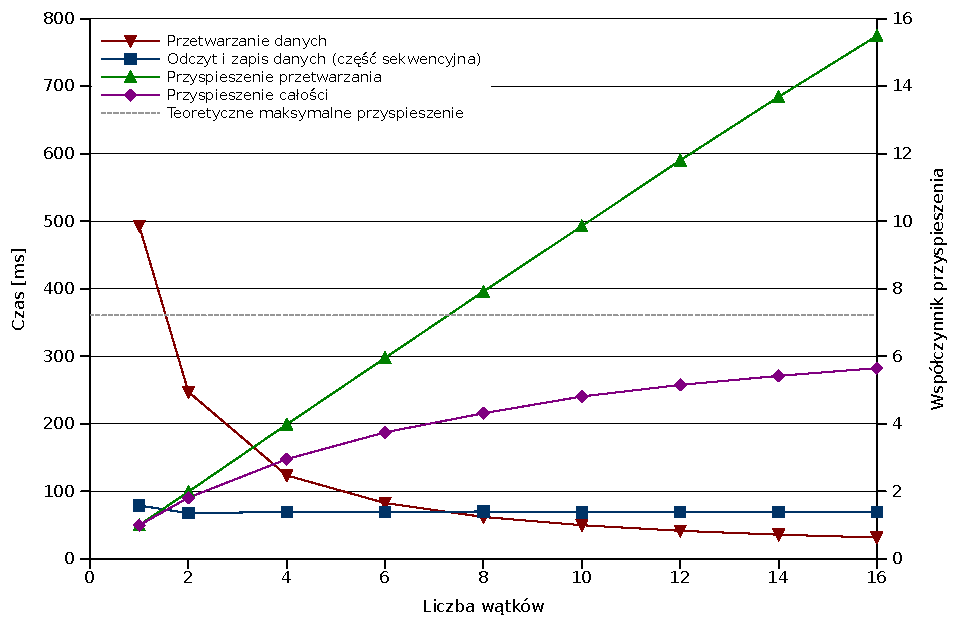
\includegraphics[width=\textwidth]{\PICSDIR/omp.pdf}
\caption{Wyniki testów wydajnościowych aplikacji zrównoleglonej przy użyciu OpenMP.}
\label{rys:res_omp}
\end{figure}

Osiągnięte wyniki są zgodne z naszymi oczekiwaniami. Widać wyraźną
zależność czasu przetwarzani danych od liczby wątków przetwarzających. Sama część
równoległa przyspiesza liniowo wraz ze wzrostem liczby wątków (przyspieszenie niemal 
16-to krotnie dla 16 wątków), część sekwencyjna wykonuje się niezależnie od liczby
wątków w tym samym czasie. Przyspieszenie całego programu także rośnie wraz ze wzrostem liczby
wątków, jednak w momencie, kiedy część sekwencyjna wykonuje się widocznie dłużej od części 
równoległej przyspieszenie dąży do wartości granicznej. Wartość tą można wyznaczyć
ze wzoru Amdahla:\\
$$ S(p) \xrightarrow[p \rightarrow \infty]{} \frac{1}{\beta(1)} $$ \\
gdzie $S(p)$ to przyspieszenie a $\beta(1)$ to udział czasu wykonania części sekwencyjnej 
w czasie wykonania całego programu w wersji 1-no wątkowej.
$$\beta(1)=\frac{T_s(1)}{T(1)}=0.138$$
$$S(p)\xrightarrow[p \rightarrow \infty]{} 7.22$$

Widać z tąd wyraźnie, że dla pliku o wielkości 10MB maksymalne możliwe do uzyskania
przyspieszenie całego procesu szyfrowania wynosi 7.22 (przerywana linia na wykresie).

\subsubsection{Wyniki -- MPI}

Poniżej przedstawione są wyniki dla wersji MPI. Testy zostały wykonane na klastrze obliczeniowym
wyposażonym w osiem maszyn z dwurdzeniowymi procesorami Intel Core2Duo E8400 2,0GHz.
Na każdej z maszyn uruchomione mogły być maksymalnie 2 procesy (po jednym na rdzeń).

W tabeli~\ref{tab:mpi}
zebrane zostały wyniki pomiarów dla pliku testowego wielkości 10MB. W~tym wypadku
mierzony był czas wykonania programu od momentu rozpoczęcia rozsyłania danych do
momentu zakończenia ich odbierania po przetworzeniu. Czas wczytywania i~zapisywania
danych na dysku nie jest uwzględniony. Oznaczenia:
\begin{itemize}
\item $p$ -- liczba procesów,
\item $T_s(p)$ -- czas komunikacji (rozesłanie i zebranie danych) przy podziale na $p$ procesów,
\item $T_p(p)$ -- czas wykonania części równoległej (szyfrowanie) przy podziale na $p$ procesów,
\item $T(p)$ -- całkowity czas szyfrowania przy podziale na $p$ procesów,
\item $E(p)$ -- wydajność samej operacji szyfrowania,
\item $S_p(p)$ -- przyspieszenie części równoległej,
\item $S(p)$ -- przyspieszenie całego algorytmu.
\end{itemize}

\begin{table}[h!]
\caption{Czas przetwarzania danych w wersji MPI}
\centering
\footnotesize
\begin{tabular}{rrrrrrr}
\toprule
$p$&$T_s(p)$&$T_p(p)$&$T(p)$&$E(p)$&$S_p(p)$&$S(p)$\\
\cmidrule{1-7}
&ms&ms&ms&MB/s&&\\
\midrule
 1 &  12,08 & 629,05 & 641,13 &  15,90 &  1,00 & 1,00 \\
 2 &  13,53 & 326,62 & 340,14 &  30,62 &  1,93 & 1,88 \\
 4 & 106,05 & 159,68 & 265,73 &  62,63 &  3,94 & 2,41 \\
 6 & 131,71 & 106,05 & 237,76 &  94,30 &  5,93 & 2,70 \\
 8 & 147,18 &  78,59 & 225,77 & 127,25 &  8,00 & 2,84 \\
10 & 460,74 &  62,91 & 523,66 & 158,95 & 10,00 & 1,22 \\
12 & 661,27 &  52,64 & 713,91 & 189,99 & 11,95 & 0,90 \\
14 & 599,26 &  44,85 & 644,11 & 222,95 & 14,00 & 1,00 \\
16 & 542,33 &  39,26 & 581,59 & 254,73 & 16,00 & 1,10 \\
\bottomrule
\end{tabular}
\label{tab:mpi}
\end{table}


\begin{figure}[h!]
\centering
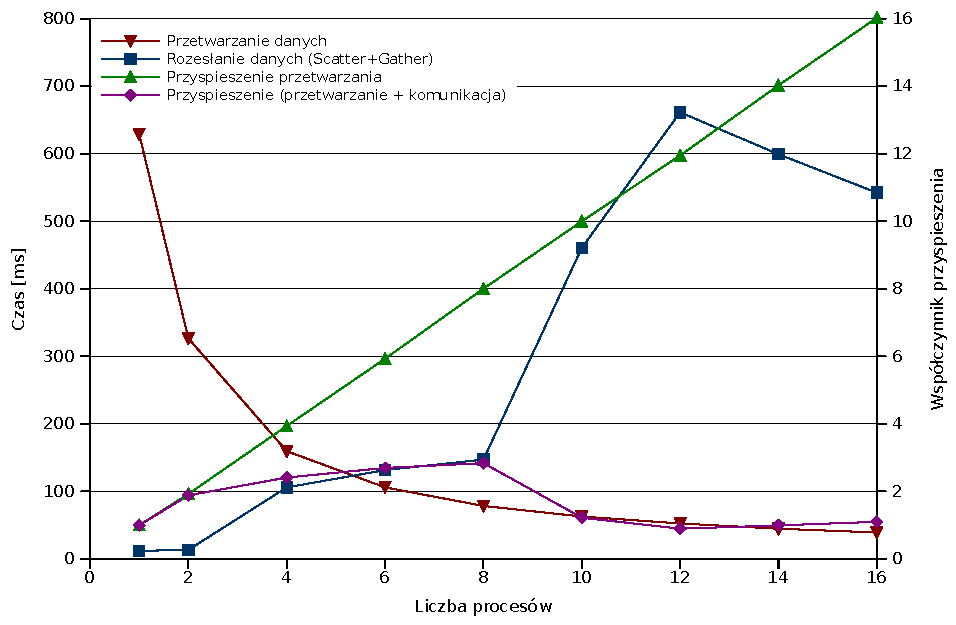
\includegraphics[width=\textwidth]{\PICSDIR/mpi.pdf}
\caption{Wyniki testów wydajnościowych aplikacji zrównoleglonej przy użyciu MPI.}
\label{rys:res_mpi}
\end{figure}

Wykres~\ref{rys:res_mpi} przedstawia w sposób obrazowy uzyskane wyniki.
W tym wypadku przyspieszenie części równoległej jest praktycznie idealne -- 16-krotne
dla 16 procesów. Jednak opóźnienia wprowadzane przez komunikację (szczególnie w momencie,
kiedy liczba procesów przekroczyła liczbę serwerów i niektóre z nich musiały odebrać 
po dwie paczki danych) powodują, że całkowite przyspieszenie nie osiąga nawet
trzykrotnej wartości programu sekwencyjnego, a w niektórych przypadkach wersja
równoległa jest nawet wolniejsza.

\subsubsection{Wnioski}
Algorytm AES w trybie CTR bardzo dobrze nadaje się do zwrównoleglania. Sama część
wykonawcza uzyskuje przyspieszenie równe ilości wątków/procesów, jednak ogólny 
wzrost wydajności ograniczony jest przez operacje wejścia/wyjścia. W obu przypadkach 
czas tych operacji zależny jest wprost od wielkości danych (większy plik dłużej się
wczytuje oraz dłużej przesyła przez sieć), tak więc efektywnie opłaca się używać
podziału na maksymalnie 6 zadań, później czas części sekwencyjnej przekracza
czas wykonania części równoległej i dalszy podział zadania traci sens. Testy wykonane
na danych o wielkości od 10 do 100MB pokazały, że w każdym wypadku czas wykonania
części równoległej w  przedstawionej implementacji po podziale na więcej niż 6 podzadań 
spada poniżej czasu operacji I/O.

Znacznie lepszym kandydatem do dużego zrównoleglania są algorytmy wykonujące bardziej
skomplikowane obliczenia na otrzymanej części danych, takie jak chociażby łamanie 
MD5 -- dane na wejściu są bardzo małe (16 bajtów), operacje są czasochłonne. W przypadku 
algorytmu AES sytuację mogłoby poprawić szyfrowanie pliku partiami wg schematu:
\begin{itemize}
\item wczytanie pierwszej porcji danych,
\item 6 wątków przetwarza wczytany blok, 7 wątek wczytuje kolejną porcję danych.
\end{itemize}
Ilość wątków moża dobrać w taki sposób, aby przetwarzanie i wczytywanie danych z dysku
miało zbliżoną prędkość (dla 6 wątków przedstawiona implementacja osiąga 120MB/s, co 
jest wartością możliwą do osiągnięcia przy odczycie przez współczesne dyski twarde).
Taka wersja implementacji powoliłaby na szyfrowanie strumienia niemalże w czasie
rzeczywistym -- jedyne opóźnienie wprowadzane byłoby przez buforowanie pierwszego bloku danych.


\end{document}

